\documentclass[11pt]{article}

% --- Geometry & layout ---------------------------------------------------
\usepackage[margin=1in]{geometry}
\usepackage{microtype}
\setlength{\parskip}{0.35em}

% --- Math ----------------------------------------------------------------
\usepackage{amsmath}
\usepackage{amssymb}

% --- Tables & figures ----------------------------------------------------
\usepackage{booktabs}
\usepackage{array}
\usepackage{graphicx}
\usepackage{caption}
\captionsetup{font=small,labelfont=bf}
\usepackage{float}

% --- Definition box ------------------------------------------------------
\usepackage[framemethod=default]{mdframed}
\newmdenv[linewidth=0.6pt,linecolor=black!55,backgroundcolor=black!3,
          innertopmargin=6pt,innerbottommargin=6pt,skipabove=6pt,skipbelow=6pt]{defbox}

% --- Links (load last) ---------------------------------------------------
\usepackage[hidelinks]{hyperref}

\title{\textbf{An Agentic AI Framework for Health Triage\\ in Low-Resource Settings}}
\author{%
\begin{tabular}{@{}*{3}{>{\centering\arraybackslash}p{0.31\textwidth}}@{}}
\textbf{Dr.~Padmanabhan Seshaiyer} & \textbf{Harisri Sanjivan S} & \textbf{Surya Thangaraju}\\[2pt]
Professor and Director, George Mason University & Software Engineer, Winter Inc & University of Pennsylvania\\[2pt]
{\footnotesize\texttt{pseshaiy@gmu.edu}} & {\footnotesize\texttt{harisri.sanjivan@peerislands.io}} & {\footnotesize\texttt{suryathangaraju04@gmail.com}}
\end{tabular}\\[1.2em]
\begin{tabular}{@{}*{2}{>{\centering\arraybackslash}p{0.36\textwidth}}@{}}
\textbf{Varun V} & \textbf{Rishi Kumar}\\[2pt]
Forward Deployed Engineer, 1hat & Forward Deployed Engineer, TH Solutions\\[2pt]
{\footnotesize\texttt{vvarun106@gmail.com}} & {\footnotesize\texttt{rishikummar10@gmail.com}}
\end{tabular}%
}
\date{October 2026}

\begin{document}
\maketitle

\begin{abstract}
\noindent
More than half the world's population --- at least 4.5~billion people --- were not fully covered by
essential health services in 2021, a gap concentrated in rural and low-resource communities~\cite{whoucov}.
Where clinicians are out of reach, the first and often decisive step in a health emergency is a judgement
made at home: whether a complaint is urgent enough to act on now, or whether it can wait. Delay in that
decision --- waiting until morning, or until a problem becomes unmistakable --- is a long-recognised and
frequently fatal failure in such settings, made with little support and no coordination between the
patient, a frontline health worker, and the facilities that might help~\cite{threedelays}. This paper
addresses that gap. We propose an \emph{agentic AI framework} for message-based health triage --- sorting
cases by how urgently they need care --- developed through a combined design-thinking and
software-engineering approach and aligned with UN Sustainable Development Goal~3. The framework coordinates
four modules over a shared, typed case record: it reads the message into a structured form, decides an
urgency level with a calibrated ability to abstain, prioritises cases, and routes urgent ones to a
suitable facility. Its defining mechanism is \emph{active follow-up}: when the system cannot yet commit, it
asks one targeted question and decides again. Here, \emph{agentic} refers to modules that sense, decide
and act in a loop --- judging when the information is sufficient, choosing the next question to ask, and
watching for emerging patterns --- rather than to a model that autonomously calls tools. A small language
model is confined to the single task it is
good at --- understanding free, code-mixed text --- while every decision is made by deterministic,
auditable logic. On a benchmark of symptom--condition cases the framework is dependable where a prompted
model alone is not, and resolves uncertainty through a short exchange of questions rather than by guessing.
Because its modules communicate only through the shared case record, the framework is also reusable and
extensible: a component can be swapped, or a new capability added, without disturbing the part that makes
the urgency decision.
\end{abstract}

\noindent\textbf{Keywords:} agentic AI, software architecture, design thinking, health triage,
active follow-up, selective prediction, low-resource settings, SDG-3.

\section{Introduction}
\label{sec:intro}
A community health worker in a village receives a message: ``the child has had fever and loose motions
for two days''. Someone must decide whether the child should be seen today, taken to a district
hospital, or cared for at home. In much of rural India that decision falls to a person with a few weeks
of training, a mobile phone, and no clinician within reach. \emph{Triage} --- sorting people by how
urgently they need care --- is the first and most consequential step in that chain, and it is precisely
where help is scarcest. Community health workers are the front line of primary care in these
settings~\cite{lewin}, and digital tools delivered over a basic phone are increasingly used to support
them~\cite{whodigital}.

This paper asks how a small language model running on ordinary hardware can support that decision, and
arrives at a clear design position: the model should \emph{read} the message, and it should not
\emph{decide} what to do about it. A language model understands a code-mixed, lay description of
symptoms remarkably well; asked instead to choose an urgency level, it is confidently unreliable
(Section~\ref{sec:eval}). Our response is to surround the model with deterministic structure so that
the strengths of each part are used and none is trusted beyond them.

We present this structure as an \emph{agentic AI framework}, and it is worth being precise about the
word. We mean \emph{agentic} in the classical sense of components that run a \emph{sense--decide--act}
loop --- perceiving the current state of a case, deciding what to do next, and acting on that decision
--- and not in the narrower, more recent sense of a language model that autonomously calls external
tools~\cite{react,toolformer,agentsurvey}. Several parts of the framework embody this loop. The reading module (Agent~1) does more than
extract fields: it judges whether the information gathered so far is enough to decide and, when it is
not, hands control to the follow-up module, which decides the single most useful question to ask, asks
it, senses the reply, and repeats until the case resolves. The surveillance module (Agent~2) runs the
same loop over the stream of incoming cases, deciding when an emerging pattern warrants an alert and
acting on it. Crucially, the decisions inside these loops are made by deterministic, auditable logic
rather than by the language model's judgement --- a deliberate safety property, not a limitation. The
modules communicate only through one shared, typed record, so the framework itself is the contribution:
its parts are standard, interchangeable choices, and dependable behaviour emerges from simple,
inspectable pieces that can be reused and extended. Figure~\ref{fig:overview} shows the framework at a
glance.

\begin{figure}[t]
\centering
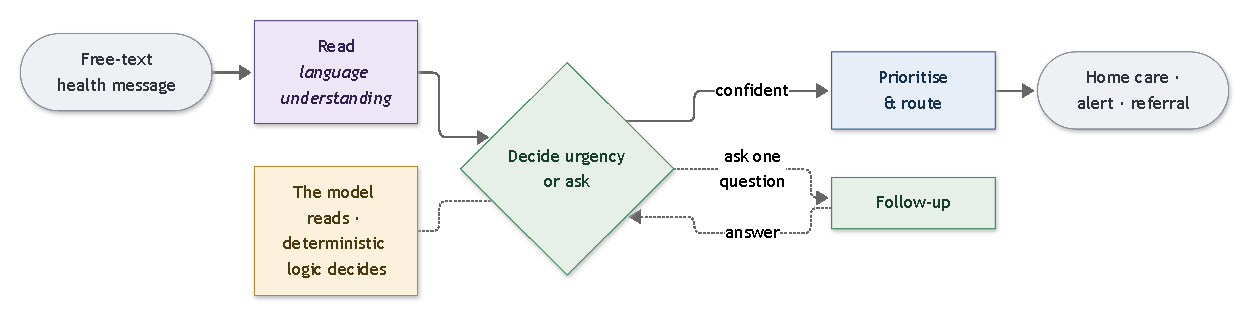
\includegraphics[width=\linewidth]{figures/fig0_overview.pdf}
\caption{The framework at a glance. A message is \emph{read} by the language component; a deterministic
core \emph{decides} the urgency or, when unsure, asks one follow-up question and decides again; confident
cases are prioritised and routed to an action. The model reads; the logic decides.}
\label{fig:overview}
\end{figure}

\begin{defbox}
\textbf{Definition (triage framework).} \emph{An agentic triage framework is a coordinated system of
bounded-responsibility modules that transforms a free-text health message into an urgency decision and
a recommended action, in which a language component is confined to interpreting the message, every
urgency decision is produced by deterministic and auditable logic, and uncertainty is resolved by
asking the sender a targeted question rather than by guessing.}
\end{defbox}

\paragraph{Central thesis.} Good software design can turn an individually unreliable AI component into a
dependable system for a real use case: by confining the model to language understanding, deciding with a
method that can decline to decide, and converting uncertainty into a question, the framework behaves
dependably where the model alone does not.

\paragraph{Research questions.}
\begin{enumerate}
\item How can a language model be composed with deterministic logic so that its language ability is used
without its judgement being trusted?
\item How should a triage system represent and act on its own uncertainty, rather than being forced into
a confident answer?
\item How can such a framework be organised so that new capabilities are added without disturbing the
part that makes the urgency decision?
\end{enumerate}

\paragraph{Objectives.} First, to propose the framework and the reasoning that leads to each of its
modules. Second, to describe each module in two registers --- the design intent, then its realisation ---
so the design is legible to engineers and non-specialists alike. Third, to demonstrate on a benchmark
that the framework is dependable, that active follow-up resolves uncertainty efficiently, and that the
design extends cleanly.

The paper is organised around the framework. Section~\ref{sec:problem} frames the problem as four
coordinated tasks. Section~\ref{sec:framework} gives the architecture. Section~\ref{sec:modules}
describes each module, design-first and then in realisation. Section~\ref{sec:application} walks a case
through the framework. Section~\ref{sec:eval} evaluates it, Section~\ref{sec:frontiers} discusses
insights and frontiers, Section~\ref{sec:related} relates it to prior work, and
Section~\ref{sec:conclusion} concludes.

\section{The problem, as four coordinated tasks}
\label{sec:problem}
We treat message-based triage not as one task but as four that must hold together
(Figure~\ref{fig:context}). Reading from the problem rather than from any solution, a usable system has
to: (i) \emph{understand} a short message written in English, a regional language, or a mixture, and turn
it into a structured account of the case; (ii) \emph{decide} an urgency level from that account, or
recognise that it cannot yet decide; (iii) \emph{prioritise} among cases that share an urgency level; and
(iv) \emph{route} urgent cases to a facility that can actually treat them.

\begin{figure}[t]
\centering
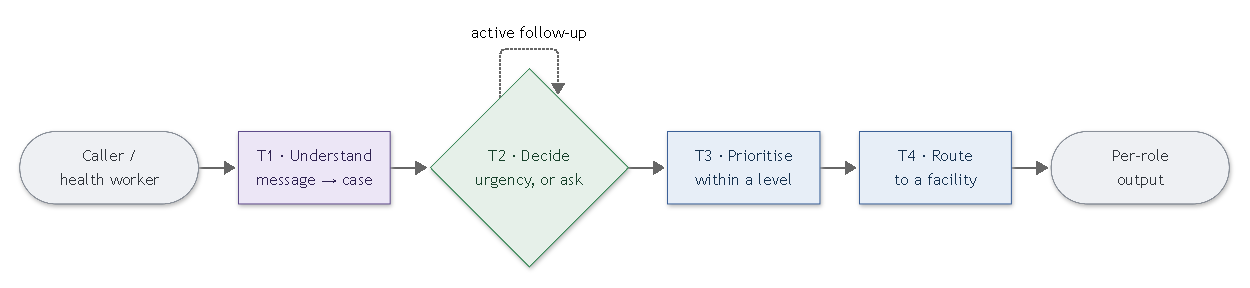
\includegraphics[width=\linewidth]{figures/fig1_context.pdf}
\caption{The problem, decomposed into four coordinated tasks. Only the reading task uses the language
model; the loop on the decision task is active follow-up, which turns ``not yet sure'' into ``ask one
question and decide again''.}
\label{fig:context}
\end{figure}

The decision task is linked to the others by one mechanism. When the system cannot commit to an urgency
level, it neither escalates blindly nor guesses: it asks the single most informative question, folds the
answer back into the case, and decides again. This \emph{active follow-up} is the idea the rest of the
framework is built to support.

\paragraph{A guiding design principle: the model reads, it does not decide.} The language model is used
only where language understanding is genuinely required --- turning a message into a structured case ---
and never for the urgency decision itself. Every decision, priority and routing choice is made by
deterministic logic that can be inspected and reproduced. This separation is the single most important
commitment in the design, and the evaluation (Section~\ref{sec:eval}) is what justifies it.

\paragraph{What ``dependable'' means here.} Throughout, we judge the framework by how it handles its own
uncertainty against the urgency levels of a demonstration benchmark, using two plain rates: the fraction
of urgent cases it surfaces at too low a level (\textbf{under-call}), and the fraction of routine cases it
surfaces at too high a level (\textbf{over-call}). These are engineering properties of the system, not
clinical judgements.

\section{The framework}
\label{sec:framework}
Figure~\ref{fig:architecture} shows the framework as four bounded-responsibility modules arranged around
a single shared record of the case. A reading module turns the message into that record; a decision module
reads the record and writes an urgency level into it; a prioritisation-and-routing module reads the decided
record and adds a recommended action. Each module speaks only through the shared record, so none reaches
into another's internals. Figure~\ref{fig:pipeline} shows the same system as a forward flow, with the two
rules that cut across it: the follow-up loop that returns to the decision module, and a safety override
that forces the highest urgency whenever a danger sign is present, on any path.

\begin{figure}[t]
\centering
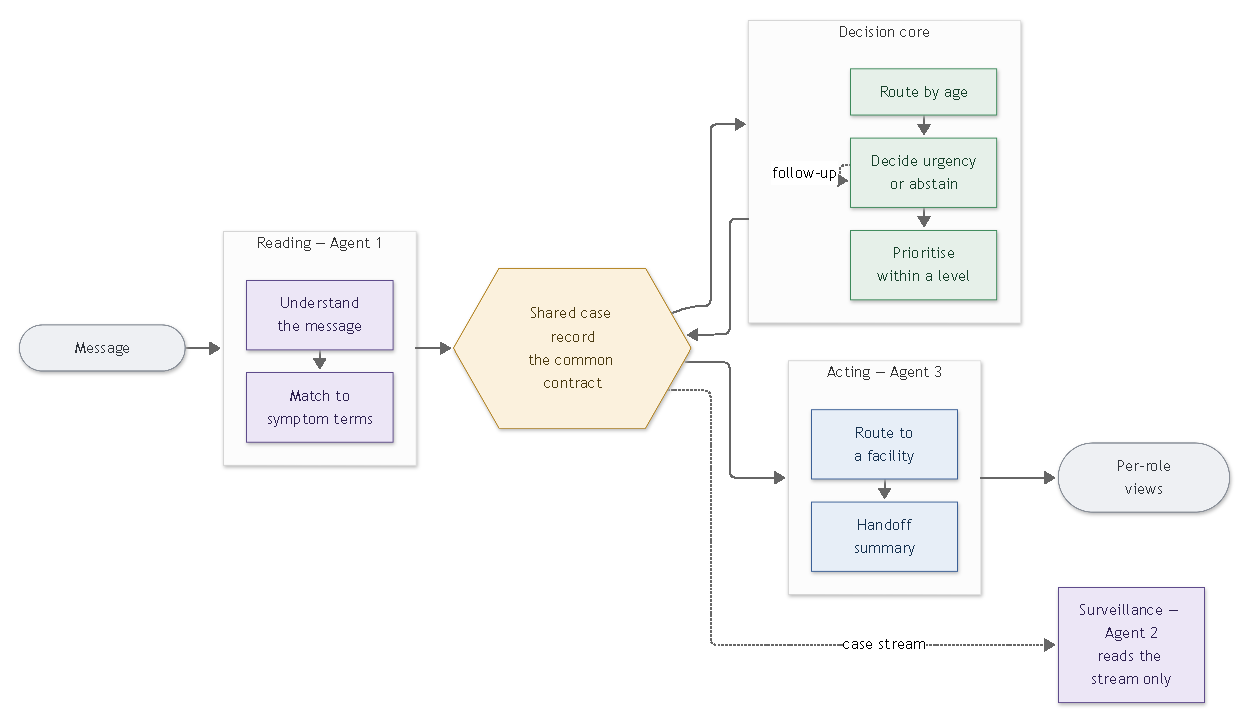
\includegraphics[width=\linewidth]{figures/fig2_architecture.pdf}
\caption{Architecture. Bounded-responsibility modules coordinate through one shared, typed case record ---
the common language every module speaks. A new capability reads the same record without touching the
decision path.}
\label{fig:architecture}
\end{figure}

\begin{figure}[t]
\centering
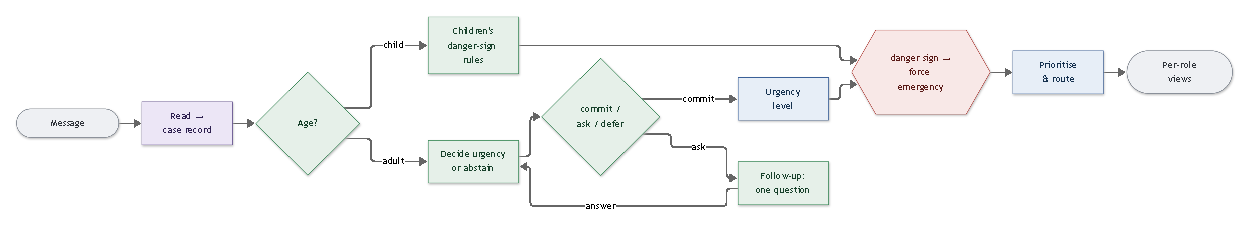
\includegraphics[width=\linewidth]{figures/fig3_pipeline.pdf}
\caption{The framework as a forward flow. The dashed arrow is active follow-up: an answer re-enters the
decision rather than being added to the output. The safety override applies on every branch.}
\label{fig:pipeline}
\end{figure}

\paragraph{The shared case record is the contract.} The one design decision that makes the framework a
framework is that every module reads and writes the same typed record (Figure~\ref{fig:dataflow}). The
record distinguishes three states for every clinical fact --- reported present, reported absent, and not
mentioned --- and nothing downstream is allowed to treat ``not mentioned'' as ``absent'', because that
would turn ``we do not know'' into ``we checked and it is fine''. Because the modules share this contract,
one can be replaced, or a new one added, without rewriting the others.

\begin{figure}[t]
\centering
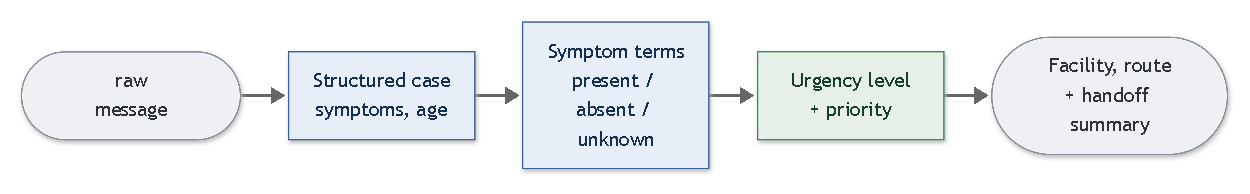
\includegraphics[width=\linewidth]{figures/fig4_dataflow.pdf}
\caption{The shared case record as it moves through the framework. Each module reads the record, adds its
own fields, and passes it on; the follow-up loop re-enters an earlier stage with one more fact known.}
\label{fig:dataflow}
\end{figure}

\section{The modules}
\label{sec:modules}
Each module is described in two registers. \emph{Design} states, from the problem, what the module must
achieve and why --- the ideation, in plain language. \emph{Realisation} then states how we build it: the
approach chosen, why it is preferred over the alternatives, and the evidence that it works. The two are
kept separate so the reasoning is never blurred with the mechanism.

\subsection{Reading the message}
\label{sec:extraction}
\paragraph{Design.} The first thing the system must do is understand a message that a worried layperson
actually writes --- short, informal, often mixing languages and scripts, naming a few symptoms rather than
a complete history. The module must turn this into a structured account the rest of the framework can act
on, and it must be careful about what it does \emph{not} know: a symptom that was never mentioned is not the
same as a symptom that was denied, and the design must preserve that difference. Reading is the one place
where genuine language understanding is unavoidable, so it is the one place the language model belongs.

\paragraph{Realisation.} We use a small, locally run language model to read the message into the structured
case record. A small model is the right choice here: it runs on the modest hardware available at the edge,
keeps data on-device, and --- as the evaluation shows --- reads code-mixed lay language~\cite{gluecos} reliably when it is
asked only to extract rather than to judge. Because free-text phrases rarely match a fixed vocabulary
exactly, each phrase is mapped to a controlled set of symptom terms by nearest-neighbour search over
multilingual sentence embeddings~\cite{msbert}, with a matching threshold calibrated on a labelled sample (97.5\% accuracy
at the chosen setting). The module confines the model to interpretation and hands on a clean, typed record.

\subsection{Deciding the urgency, or declining to}
\label{sec:gate}
\paragraph{Design.} Given the structured case, the system must decide an urgency level --- but a responsible
triage design must also be allowed to say ``not yet''. Forcing a single answer on thin evidence is exactly
how an automated system becomes unsafe. So the decision module is built around an idea stronger than a best
guess: it should hold a small set of plausible conditions, commit only when that set points to one answer,
and otherwise either ask for more information or defer. When it must act under remaining uncertainty, it
should err toward caution --- treat the case as the most serious possibility still in play --- so that an
urgent case is never quietly surfaced as a routine one.

\paragraph{Realisation.} Adult cases are decided by a Naive Bayes classifier over the benchmark conditions.
We prefer Naive Bayes here deliberately: on the short, few-symptom messages this use case actually produces
it is both more accurate and far better calibrated than richer alternatives such as logistic regression,
which is overconfident and brittle on such sparse input --- and calibration is what the rest of the design
depends on. Rather than take the classifier's single best guess, we wrap it in \emph{conformal prediction},
a standard selective-prediction method that returns a \emph{set} of plausible conditions with a tunable
guarantee on how often the true condition is inside it. The size of that set becomes the decision
(Figure~\ref{fig:gate}): one condition means commit; a few means stay uncertain and ask; many means defer.
When the set holds more than one, the system labels the case with the most serious urgency level present in
it --- the one rule that converts the set guarantee into a guarantee about the urgency the health worker
sees. A danger-sign override sits above all of this and forces the highest urgency directly. Paediatric
cases follow a small, separate set of danger-sign rules~\cite{who} rather than the classifier.

\begin{figure}[t]
\centering
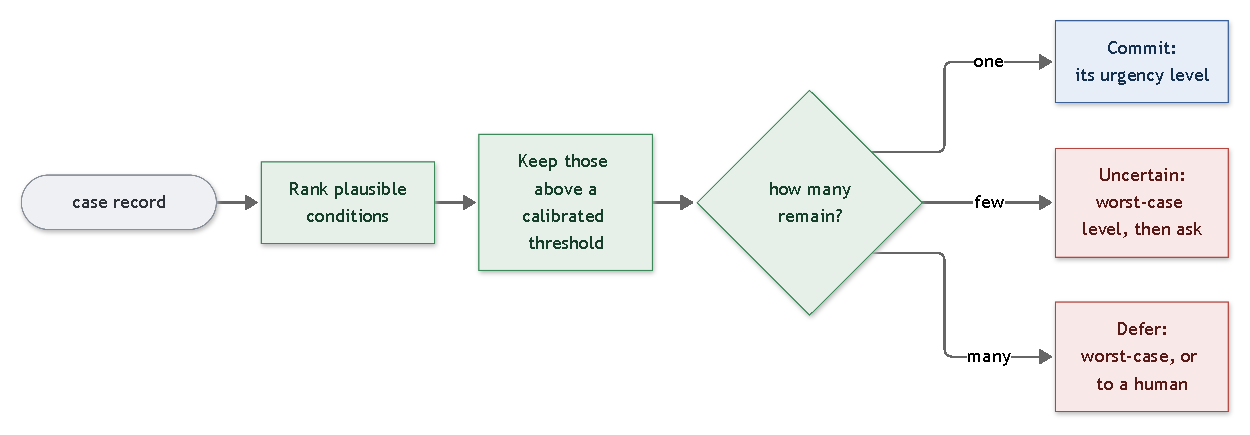
\includegraphics[width=\linewidth]{figures/fig5_gate.pdf}
\caption{The decision module. The \emph{size} of the plausible-condition set, not its contents, chooses the
next action: commit, ask, or defer. Labelling an uncertain case by its most serious possibility is what
keeps an urgent case from being under-called.}
\label{fig:gate}
\end{figure}

\subsection{Active follow-up: turning uncertainty into a question}
\label{sec:followup}
\paragraph{Design.} This is the mechanism that defines the framework. When the decision module cannot yet
commit, the natural human move is not to escalate everything to be safe, nor to guess, but to \emph{ask one
more thing}. A good design asks the \emph{single most useful} question --- the one whose answer, either way,
would most reduce the remaining uncertainty --- phrases it in the sender's own language, and must never
invent an answer: a hedge or an unclear reply is re-asked, not coerced. A ``no'' must be as informative as a
``yes'', because knowing what the patient does \emph{not} have is often what separates two conditions. The
exchange should be short, and should stop as soon as the case is resolved.

\paragraph{Realisation.} The question is \emph{selected} by deterministic reasoning over the current set of
plausible conditions, choosing the symptom whose presence or absence would most shrink that set; the language
model only phrases the chosen question, so the policy itself is fully auditable and does not depend on the
model's judgement (Figure~\ref{fig:followup}). The reply is read as yes, no, or unclear, and an unclear reply
is re-asked. Crucially, a denial is fed back as genuine evidence --- treating ``no'' as informative is what
makes the exchange efficient: in evaluation the system resolves 74.8\% of initially uncertain cases, in a mean
of about two questions, and over-calls fall sharply as a result. The loop stops when the case resolves to a
single condition, a small question budget is spent, or no useful question remains.

\begin{figure}[t]
\centering
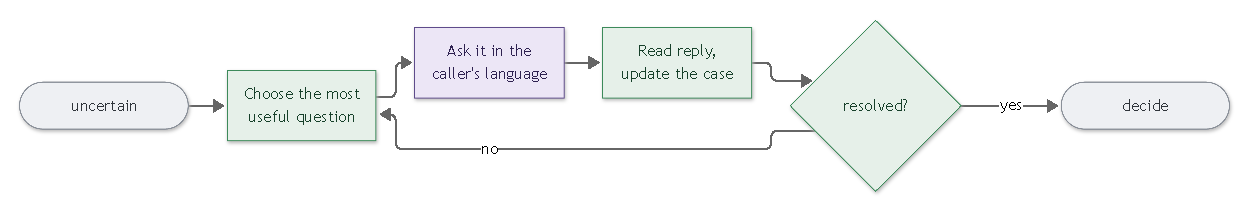
\includegraphics[width=\linewidth]{figures/fig6_followup.pdf}
\caption{Active follow-up. The question is selected deterministically and only phrased by the model; a
``yes'' and a ``no'' are equally informative; a hedge is re-asked; the decision is then re-made.}
\label{fig:followup}
\end{figure}

\subsection{Prioritising and routing}
\label{sec:routing}
\paragraph{Design.} Two cases can share an urgency level and still not be equally pressing, so the system
must order cases \emph{within} a level for attention. And for the urgent ones it must point to a facility
that can actually help --- one that can treat the case, is open, and is reachable --- rather than simply the
nearest. The output must be shaped for whoever reads it: a caller, a health worker, a receiving clinician.

\paragraph{Realisation.} Within a level, cases are ordered by a transparent multi-criteria score (an
Analytic Hierarchy Process) over clinically meaningful attributes such as complication risk, time
sensitivity and transmissibility, with the attribute weights derived from pairwise comparisons rather than
set by hand. This ordering never changes the urgency level; it only sequences cases that share one. Routing
filters candidate facilities by what the case needs and then selects by travel distance, behind an interface
that can use an offline estimate or a real routing service. A concise handoff summary is produced for the
receiving clinician.

\subsection{An illustrative extension}
\label{sec:extension}
Because every module speaks through the shared case record, a new capability can read that same record
without touching the decision path. As a demonstration, we added an outbreak-surveillance capability that
watches the stream of recorded cases for unusual local clusters and raises an alert with a recommended
action (Figure~\ref{fig:extension}, Table~\ref{tab:extensibility}). It was built against the shared record
alone, made no change to the modules that decide urgency, and is kept from depending on the decision logic
by an automated check. That a second capability could be added this cleanly is a practical property of the
design, shown here rather than merely asserted.

\begin{figure}[t]
\centering
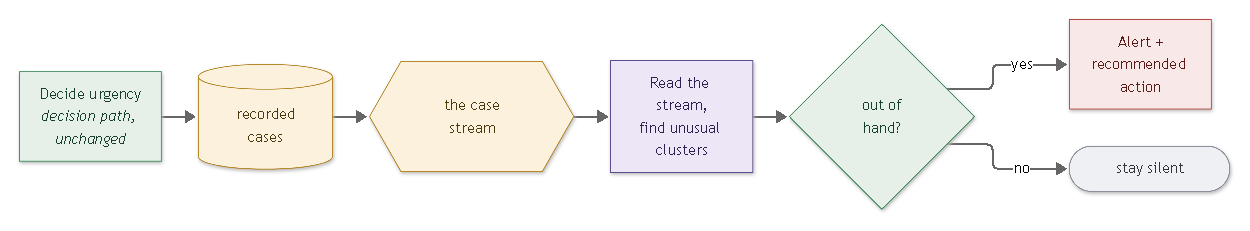
\includegraphics[width=\linewidth]{figures/fig7_extension.pdf}
\caption{Adding a capability through the shared record. The surveillance module reads the case stream and
depends on none of the decision logic, so it extends the framework without disturbing it.}
\label{fig:extension}
\end{figure}

\begin{table}[h]
\centering
\caption{Adding a capability without touching the decision path.}
\label{tab:extensibility}
\small
\begin{tabular}{p{8.5cm}p{5.5cm}}
\toprule
Property & Observed \\
\midrule
Changes to the urgency-decision path & none \\
How it reads data & through the shared case record only \\
Dependence on the decision logic & none (checked automatically) \\
Additional changes required & a reader view and one optional field \\
Alert on a stream containing one injected outbreak & raised, correctly \\
Alert on a stream with no outbreak & none \\
\bottomrule
\end{tabular}
\end{table}

\section{An illustrative application}
\label{sec:application}
To show the framework at work, consider a caregiver's message: ``child, fever and loose motions for two
days''. The reading module turns it into a structured case with two symptoms present and the child's
age noted. The decision module finds several childhood conditions consistent with so little information
and does not commit. Active follow-up asks the single most useful question --- whether the child is able
to drink --- phrased in the caregiver's language. The answer ``no'' is strong evidence: it both narrows the
plausible conditions and, as a danger sign, triggers the safety override. The case is surfaced as an
emergency, prioritised above less time-sensitive cases at the same level, and routed to the nearest facility
able to manage a child in that state, with a short summary for the receiving clinician.

The same path handles easier cases with less work. A message describing a mild, self-limiting complaint
resolves to a single low-urgency condition on the first pass, with no questions asked and advice to care at
home. A message that is genuinely ambiguous is carried by follow-up: two or three questions typically move it
from a wide set of possibilities to a single decision, and where they cannot, the system defers to a human
rather than guessing. In each case the language model only reads and phrases; the urgency is decided by logic
that can be inspected after the fact.

\section{Evaluation}
\label{sec:eval}
We evaluate how the framework handles its own uncertainty on a demonstration benchmark of symptom--condition
cases spanning 41 conditions. The benchmark is used as a controlled sandbox in which the framework's behaviour
can be observed free of real-world confounders; real-world clinical validation is future work
(Section~\ref{sec:frontiers}). Each case is presented to the system as the few symptoms a person would
actually mention, with the full case held back as ground truth, and the framework is evaluated out-of-sample.

Before the numbers, Table~\ref{tab:comparison} summarises what separates the framework from the two obvious
alternatives --- prompting the model directly, and a plain best-guess classifier --- along the properties
this section measures. The findings then answer the three research questions of Section~\ref{sec:intro}: that
composing the model with deterministic logic uses its language ability without trusting its judgement; that
the system represents and acts on its own uncertainty rather than being forced into an answer; and that it
extends without disturbing the decision.

\begin{table}[t]
\centering
\caption{What each approach provides. Only the framework offers every property; the measured differences are
quantified in the tables and charts that follow.}
\label{tab:comparison}
\small
\begin{tabular}{p{7.1cm}ccc}
\toprule
Property & Prompted model & Plain classifier & Framework \\
\midrule
Reads code-mixed free text & \checkmark & $\times$ & \checkmark \\
Holds uncertainty as a set, not one guess & $\times$ & $\times$ & \checkmark \\
Can decline to decide (abstain or defer) & $\times$ & $\times$ & \checkmark \\
Asks a targeted follow-up question & $\times$ & $\times$ & \checkmark \\
Keeps urgent cases from being under-called & $\times$ & $\sim$ & \checkmark \\
Decision is deterministic and auditable & $\times$ & \checkmark & \checkmark \\
Extensible with new capabilities & $\times$ & $\times$ & \checkmark \\
\bottomrule
\end{tabular}

\vspace{2pt}
{\footnotesize \checkmark~provides it \quad $\sim$~partially \quad $\times$~does not}
\end{table}

\paragraph{A prompted model alone is not enough.} Asked directly to choose an urgency level with a safety
instruction in its prompt, the language model collapses onto one answer: it labels most cases ``severe'',
under-calls one in six genuinely urgent cases, and over-calls the large majority of routine ones
(Table~\ref{tab:llmonly}, Figures~\ref{fig:naive} and~\ref{fig:chartD}). The output is always well-formed; the failure is in the
decision, not the format. This is the motivation for the framework, and the reason the model is confined to
reading.

\begin{figure}[ht]
\centering
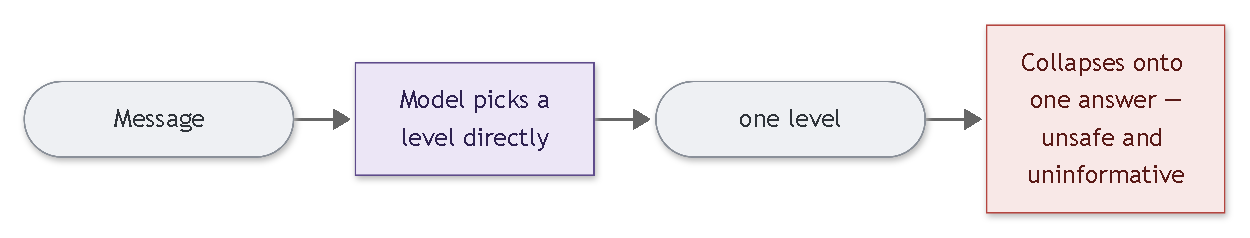
\includegraphics[width=0.9\linewidth]{figures/fig8_naive.pdf}
\caption{Why a prompted model alone is not enough: asked to decide, it collapses onto one answer and is at
once unsafe and uninformative. This motivates surrounding the model with structure.}
\label{fig:naive}
\end{figure}

\begin{table}[h]
\centering
\caption{A prompted model alone versus the full framework, on the same cases.}
\label{tab:llmonly}
\small
\begin{tabular}{lcc}
\toprule
System & under-call $\downarrow$ & over-call $\downarrow$ \\
\midrule
Prompted model alone (with a safety instruction) & 0.169 & 0.827 \\
The framework (shipped, with follow-up) & 0.021 & 0.056 \\
\bottomrule
\end{tabular}
\end{table}

\begin{figure}[tb]
\centering
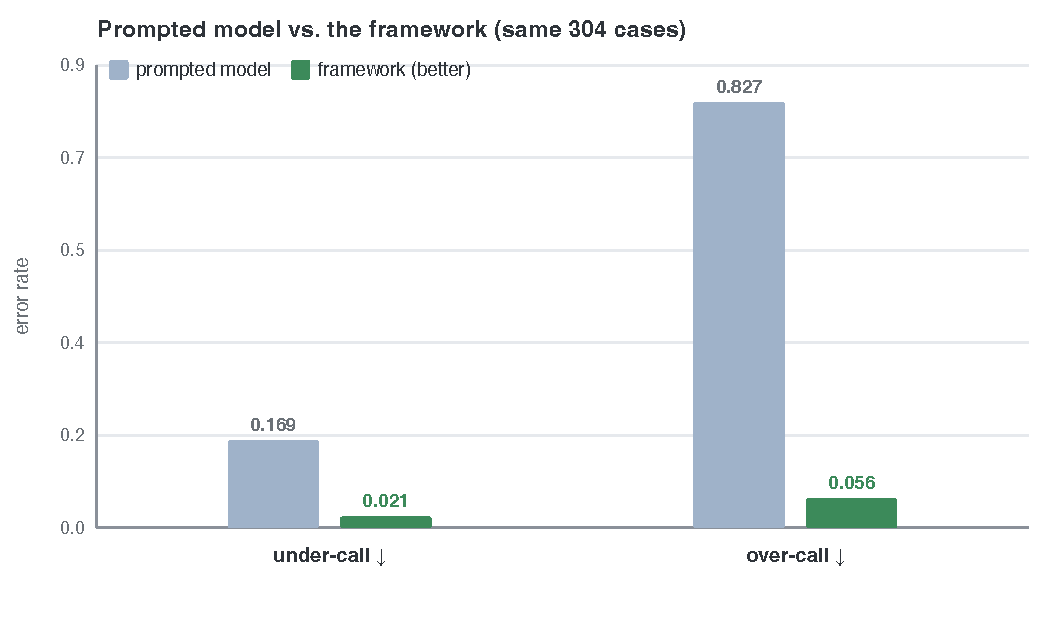
\includegraphics[width=0.82\linewidth]{figures/chartD.pdf}
\caption{The prompted model versus the shipped framework on the same 304 cases: the framework makes far
fewer under-calls (2.1\% against 16.9\%) and far fewer over-calls (5.6\% against 82.7\%).}
\label{fig:chartD}
\end{figure}

\paragraph{Structure makes the system dependable, step by step.} Adding the framework's elements one at a
time removes the failure and shows where dependability comes from (Table~\ref{tab:journey},
Figures~\ref{fig:chartA} and~\ref{fig:chartB}). A structured
decision replaces most of the prompted model's error; the ability to abstain removes more; labelling an
uncertain case by its most serious possibility removes the remaining under-calls, at the cost of caution;
and active follow-up then buys that caution back. The low under-call rate is a design property rather than a
coincidence: an uncertain case is labelled by its most serious possibility, so an urgent case is missed only
when the true condition falls outside the prediction set --- a rate the decision gate controls. Worst-case
labelling alone drives it to zero on this benchmark; the shipped system's 2.1\% is the small residual that
remains once adaptive follow-up is added.

\begin{table}[h]
\centering
\caption{Building the framework one element at a time. Each row adds one element to the row above.}
\label{tab:journey}
\small
\begin{tabular}{lcc}
\toprule
Configuration & under-call $\downarrow$ & over-call $\downarrow$ \\
\midrule
Prompted model alone & 0.169 & 0.827 \\
\;+ structured decision & 0.092 & 0.068 \\
\;+ ability to abstain & 0.063 & 0.068 \\
\;+ cautious labelling of uncertain cases & 0.000 & 0.216 \\
\;+ active follow-up (full framework) & 0.021 & 0.056 \\
\bottomrule
\end{tabular}
\end{table}

\begin{figure}[tb]
\centering
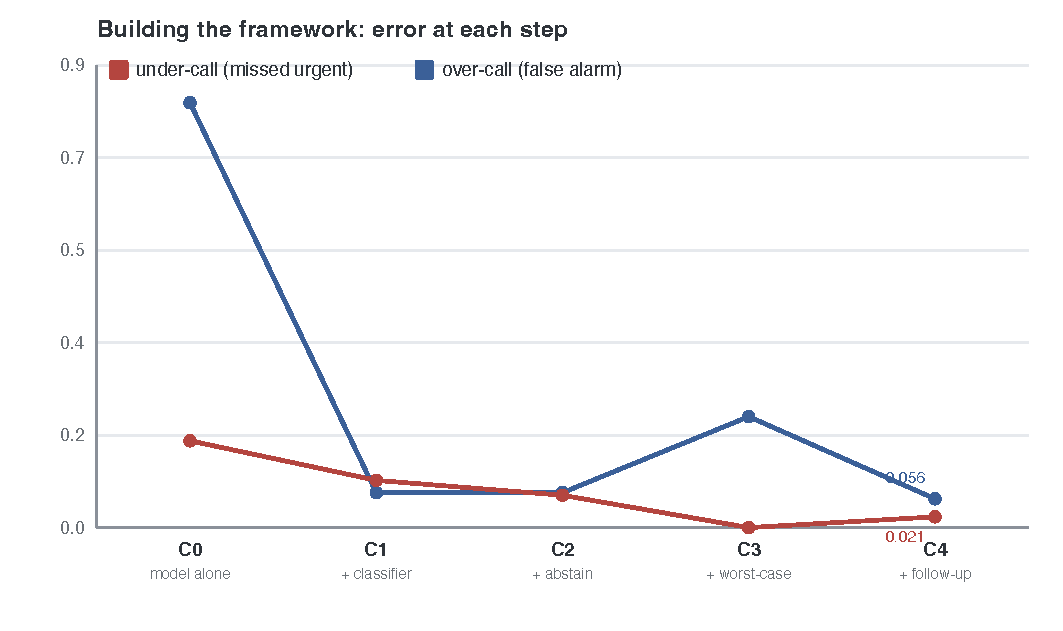
\includegraphics[width=0.84\linewidth]{figures/chartA.pdf}
\caption{Error at each build-up step. Over-call falls sharply once structure replaces the prompted model,
rises when cautious labelling drives under-call to zero, and is then bought back by active follow-up;
under-call stays low throughout.}
\label{fig:chartA}
\end{figure}

\begin{figure}[tb]
\centering
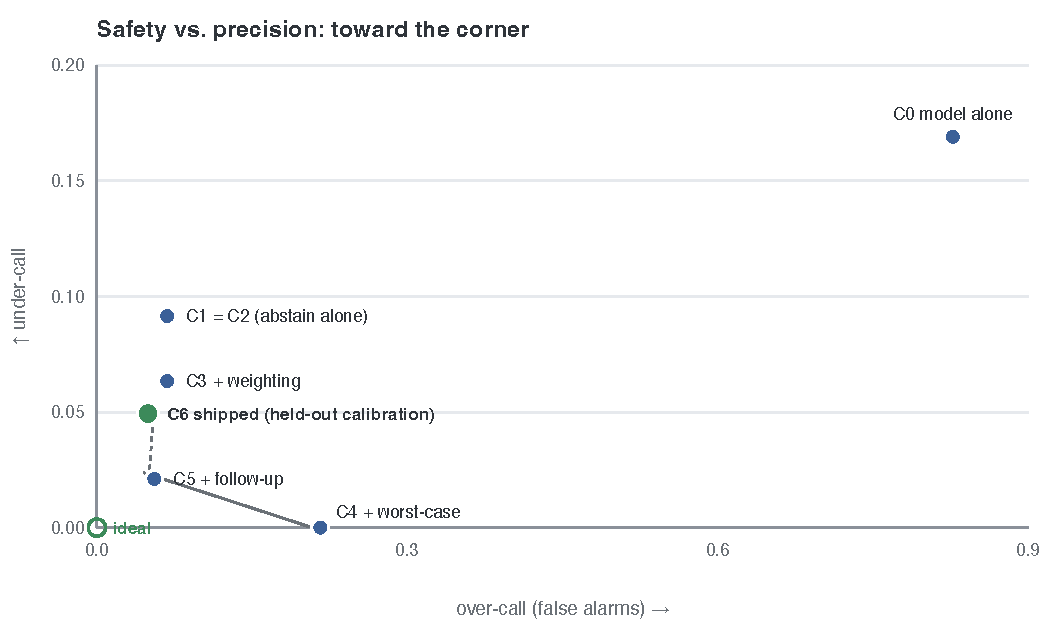
\includegraphics[width=0.74\linewidth]{figures/chartB.pdf}
\caption{The same configurations in error space. The design moves toward the ideal corner --- no missed
urgent cases, no false alarms --- and active follow-up carries the full system from the cautious point close
to it.}
\label{fig:chartB}
\end{figure}

\paragraph{Active follow-up resolves uncertainty efficiently.} The exchange of questions is where the
framework recovers precision without sacrificing safety. Treating a denial as evidence is decisive: with it,
a deterministic, most-informative question policy resolves 74.8\% of initially uncertain cases to a single
condition in a mean of about two questions, and clearly outperforms simpler question strategies
(Table~\ref{tab:followup}, Figure~\ref{fig:chartC}). The practical effect is a favourable trade: over-calls fall from 21.6\% to 5.6\%
because resolved cases no longer need cautious escalation, while under-calls stay within the designed bound.

\begin{table}[h]
\centering
\caption{Active follow-up. ``Resolved'' is the fraction of initially uncertain cases ending at a single
condition. Using a denial as evidence is what makes the exchange efficient.}
\label{tab:followup}
\small
\begin{tabular}{lccc}
\toprule
Question policy & Resolved & Mean questions & over-call $\downarrow$ \\
\midrule
Most-frequent symptom & 0.427 & 2.62 & 0.105 \\
Random useful symptom & 0.583 & 2.45 & 0.086 \\
Most-informative symptom (ours) & \textbf{0.748} & \textbf{2.15} & \textbf{0.056} \\
\bottomrule
\end{tabular}
\end{table}

\begin{figure}[tb]
\centering
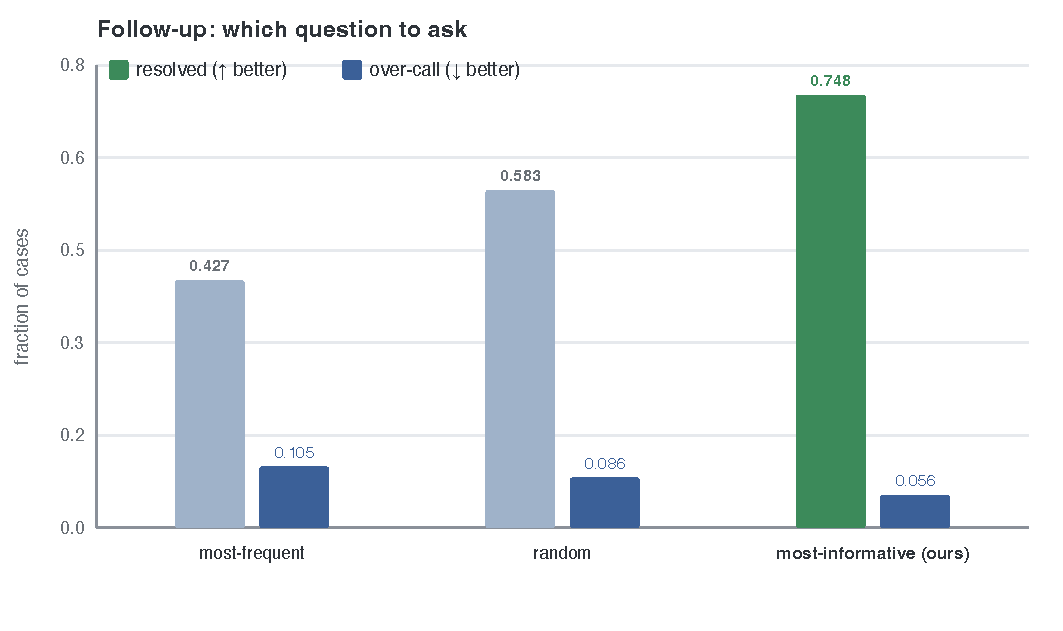
\includegraphics[width=0.82\linewidth]{figures/chartC.pdf}
\caption{Question-selection policies. Choosing the most informative question resolves far more uncertain
cases than the simpler strategies, and at the lowest over-call.}
\label{fig:chartC}
\end{figure}

\paragraph{The decision holds through real, lay language.} Run end to end from rendered messages rather than
from clean symptom lists --- including messages rewritten as real caregivers phrase them, mixing English and a
regional language --- the framework preserves its safety behaviour, at a modest cost in precision
(Appendix~\ref{app:endtoend}). The safety behaviour that holds on clean input survives the messy input the
system will actually meet.

\paragraph{The design extends cleanly.} The surveillance capability of Section~\ref{sec:extension} was added
through the shared record with no change to the decision path and no dependence on the decision logic
(Table~\ref{tab:extensibility}), and it raises an alert exactly when a cluster is present and stays silent
otherwise. The framework is a base others can build on, not a single fixed application.

\section{Design insights, reflections, and frontiers}
\label{sec:frontiers}
\paragraph{Dependability comes from the plainest rule.} The element that carries the safety result is not an
elaborate one: it is the simple rule of labelling an uncertain case by its most serious remaining
possibility. The lesson we draw is that in a composed system the guarantee should be traced back to the exact
rule that produces it, and that rule is often the simplest one in sight.

\paragraph{The whole is what must be measured.} A question-selection policy and a decision method can each be
sound in isolation and still work poorly together if one component's assumptions are not honoured by the
other; it is measuring the composed loop, not the parts, that reveals this. We therefore treat the coordinated
behaviour of the modules --- not any single module --- as the object to evaluate and to design.

\paragraph{The model is a reader, not a decider.} The evaluation makes the division of labour concrete: the
language model reads messy, code-mixed language well, and decides urgency badly. A framework that assigns the
model only the first role, and deterministic logic the second, uses each where it is strong. This is the
general principle we would carry to other high-stakes, language-fronted tasks.

\paragraph{Frontiers and future work.} The framework is demonstrated on a benchmark, not on patients, and its
urgency levels are a demonstration scale; anchoring them to a recognised clinical standard~\cite{esi} with clinician
oversight, and validating on real presentations, is the first and most important next step. Beyond it: a live
messaging channel behind the existing answer interface; automatic fallback when the local model is
unavailable; real road-network routing through the existing routing interface; a fuller paediatric ruleset;
and growing the surveillance capability from a working skeleton into an evaluated module. Each is a change at an
existing seam of the framework, which is the point of building it this way.

\section{Related work}
\label{sec:related}
\paragraph{Symptom checkers and language models for triage.} Symptom checkers have been audited against
clinician judgement for over a decade, and were found to be correct about half the time and consistently
risk-averse~\cite{semigran}. A prompted language model reproduces that risk-averse collapse in a newer
technology, but without even being safely conservative. Machine-learning triage models can outperform standard
acuity scales~\cite{levin}, and large language models perform strongly on medical-knowledge tasks~\cite{singhal,thirun};
what stays hard is turning that into a calibrated, auditable decision. Our position is not that language models
should be kept out of triage, but that they should read rather than decide.

\paragraph{Selective prediction and set-valued decisions.} The idea that a classifier should be allowed to
abstain goes back to the reject option~\cite{chow} and has a modern form for neural models~\cite{geifman}.
Conformal prediction~\cite{vovk,angelopoulos} provides set-valued predictions with a distribution-free
guarantee; the least-ambiguous-set construction we use is from Sadinle et al.~\cite{sadinle}. Our contribution
is not a new method but a way of \emph{acting} on the size of the predicted set, used as a design rule for
triage.

\paragraph{Multi-criteria prioritisation.} The Analytic Hierarchy Process~\cite{saaty} is a standard
multi-criteria method; we use it only to order cases within an urgency level, deriving its weights from
pairwise comparisons.

\paragraph{Structuring language-model systems.} Confining a language model to a well-typed boundary with
deterministic logic on either side is established engineering practice; a parallel line of work instead gives
the model agency, letting it reason and act or call external tools~\cite{react,toolformer,agentsurvey}. Our
contribution is a worked account
of where, in one such system for a real use case, the dependability actually comes from, and of an
architecture that lets the system be reused and extended.

\section{Conclusion}
\label{sec:conclusion}
A small language model can read a code-mixed health message well and cannot be trusted to decide what to do
about it. The framework proposed here keeps the model in the first role and surrounds it with deterministic
structure for the second: a shared case record that distinguishes ``absent'' from ``unknown'', a decision
that can abstain, cautious labelling that turns uncertainty into a safe urgency level, and a follow-up loop
that asks one question when the system is unsure and then decides again. On a demonstration benchmark the
framework is dependable where a prompted model alone is not, resolves most uncertain cases with a short
exchange of questions, and accepts a new capability without disturbing the decision path. Answering the
research questions of Section~\ref{sec:intro}, it composes a language model with deterministic logic so that
only its language ability is relied upon, represents and acts on its own uncertainty rather than being forced
into an answer, and is organised so that it can grow at its seams. The dataset is a demonstration benchmark
and the next step is a clinician: the framework is offered as a practical, extensible basis for AI-assisted
triage in low-resource settings, in service of SDG-3~\cite{un2030}.

\section*{Reproducibility}
The framework, its modules, and every evaluation harness are implemented in a public code repository; each
number reported here is regenerated by a scripted harness, and the deterministic harnesses reproduce
identically on every run.

\begin{thebibliography}{22}
\bibitem{whoucov} World Health Organization and World Bank. \emph{Tracking Universal Health Coverage: 2023
Global Monitoring Report}. World Health Organization and World Bank, Geneva, 2023.
\bibitem{threedelays} S.~Thaddeus and D.~Maine. Too far to walk: maternal mortality in context.
\emph{Social Science \& Medicine}, 38(8):1091--1110, 1994.
\bibitem{sadinle} M.~Sadinle, J.~Lei, and L.~Wasserman. Least ambiguous set-valued classifiers with bounded
error levels. \emph{Journal of the American Statistical Association}, 114(525):223--234, 2019.
\bibitem{vovk} V.~Vovk, A.~Gammerman, and G.~Shafer. \emph{Algorithmic Learning in a Random World}. Springer,
2005.
\bibitem{angelopoulos} A.~N.~Angelopoulos and S.~Bates. A gentle introduction to conformal prediction and
distribution-free uncertainty quantification. arXiv:2107.07511, 2021.
\bibitem{chow} C.~K.~Chow. On optimum recognition error and reject tradeoff. \emph{IEEE Transactions on
Information Theory}, 16(1):41--46, 1970.
\bibitem{geifman} Y.~Geifman and R.~El-Yaniv. Selective classification for deep neural networks. In
\emph{Advances in Neural Information Processing Systems 30}, 2017.
\bibitem{saaty} T.~L.~Saaty. \emph{The Analytic Hierarchy Process}. McGraw-Hill, 1980.
\bibitem{who} World Health Organization. \emph{Integrated Management of Childhood Illness: Chart Booklet}.
WHO, Geneva, 2014.
\bibitem{esi} N.~Gilboy, P.~Tanabe, D.~Travers, and A.~M.~Rosenau. \emph{Emergency Severity Index (ESI): A
Triage Tool for Emergency Department Care, Version 4}. Agency for Healthcare Research and Quality, 2012.
\bibitem{semigran} H.~L.~Semigran, J.~A.~Linder, C.~Gidengil, and A.~Mehrotra. Evaluation of symptom checkers
for self diagnosis and triage: audit study. \emph{BMJ}, 351:h3480, 2015.
\bibitem{un2030} United Nations General Assembly. \emph{Transforming our World: the 2030 Agenda for
Sustainable Development}. Resolution A/RES/70/1, 2015.
\bibitem{whodigital} World Health Organization. \emph{WHO Guideline: Recommendations on Digital Interventions
for Health System Strengthening}. WHO, Geneva, 2019.
\bibitem{lewin} S.~Lewin, S.~Munabi-Babigumira, C.~Glenton, et al. Lay health workers in primary and community
health care for maternal and child health and the management of infectious diseases. \emph{Cochrane Database
of Systematic Reviews}, (3):CD004015, 2010.
\bibitem{singhal} K.~Singhal, S.~Azizi, T.~Tu, et al. Large language models encode clinical knowledge.
\emph{Nature}, 620(7972):172--180, 2023.
\bibitem{thirun} A.~J.~Thirunavukarasu, D.~S.~J.~Ting, K.~Elangovan, L.~Gutierrez, T.~F.~Tan, and
D.~S.~W.~Ting. Large language models in medicine. \emph{Nature Medicine}, 29(8):1930--1940, 2023.
\bibitem{levin} S.~Levin, M.~Toerper, E.~Hamrock, et al. Machine-learning-based electronic triage more
accurately differentiates patients with respect to clinical outcomes compared with the Emergency Severity
Index. \emph{Annals of Emergency Medicine}, 71(5):565--574, 2018.
\bibitem{react} S.~Yao, J.~Zhao, D.~Yu, N.~Du, I.~Shafran, K.~Narasimhan, and Y.~Cao. ReAct: Synergizing
reasoning and acting in language models. In \emph{International Conference on Learning Representations}, 2023.
\bibitem{toolformer} T.~Schick, J.~Dwivedi-Yu, R.~Dess\`i, et al. Toolformer: Language models can teach
themselves to use tools. arXiv:2302.04761, 2023.
\bibitem{agentsurvey} L.~Wang, C.~Ma, X.~Feng, et al. A survey on large language model based autonomous
agents. \emph{Frontiers of Computer Science}, 18(6):186345, 2024.
\bibitem{msbert} N.~Reimers and I.~Gurevych. Making monolingual sentence embeddings multilingual using
knowledge distillation. In \emph{Proceedings of EMNLP}, pages 4512--4525, 2020.
\bibitem{gluecos} S.~Khanuja, S.~Dandapat, A.~Srinivasan, S.~Sitaram, and M.~Choudhury. GLUECoS: An evaluation
benchmark for code-switched NLP. In \emph{Proceedings of ACL}, pages 3575--3585, 2020.
\end{thebibliography}

\clearpage
\appendix
\renewcommand{\thetable}{A\arabic{table}}
\setcounter{table}{0}

\section{Sensitivity of the safety behaviour}
\label{app:sensitivity}
The decision module has one free setting that trades caution against commitment. Table~\ref{tab:alpha} varies
it across its range. The safety behaviour --- surfacing no urgent case at too low a level --- holds throughout,
while the setting controls how often the system commits versus asks. These figures isolate the decision gate
before active follow-up, as in the worst-case-labelling step of Table~\ref{tab:journey}; the shipped system,
which adds follow-up, is the 2.1\% of Table~\ref{tab:llmonly}. This confirms that the trade-off is a
designed dial that behaves predictably, rather than a value that has to be tuned to make the system work.

\begin{table}[h]
\centering
\caption{Varying the one free setting of the decision module. The safety behaviour holds across the range.}
\label{tab:alpha}
\small
\begin{tabular}{lccc}
\toprule
Setting & under-call & over-call & commits \\
\midrule
most cautious & 0.000 & 0.173 & 0.69 \\
intermediate & 0.000 & 0.216 & 0.66 \\
most committing & 0.000 & 0.265 & 0.58 \\
\bottomrule
\end{tabular}
\end{table}

\section{End to end, from real messages}
\label{app:endtoend}
Table~\ref{tab:endtoend} runs the whole framework from rendered messages rather than clean symptom lists,
including messages rewritten as real caregivers phrase them across English and a regional language. The
decision gate's safety behaviour survives real extraction; the cost of reading real language is a modest loss
of precision.

\begin{table}[h]
\centering
\caption{The framework run end to end from messages. ``Lay, code-mixed'' replaces each symptom with a real
caregiver phrasing across two languages.}
\label{tab:endtoend}
\small
\begin{tabular}{lccc}
\toprule
Input & understood correctly & under-call & over-call cost \\
\midrule
clean English (ceiling) & 0.99 & 0.000 & $-0.01$ \\
lay, code-mixed & 0.96 & 0.000 & $+0.05$ \\
\bottomrule
\end{tabular}
\end{table}

\section{Robustness of the message-facing behaviour}
\label{app:robustness}
Table~\ref{tab:robustness} reports how stable the framework's decisions are to how a message is written and
how reliably the follow-up exchange is understood.

\begin{table}[h]
\centering
\caption{Robustness to phrasing and reliability of the follow-up exchange.}
\label{tab:robustness}
\small
\begin{tabular}{p{11cm}r}
\toprule
Property & Result \\
\midrule
Same message submitted repeatedly, same decision & 1.000 \\
Different real phrasings of the same content, same decision & 0.750 \\
A different few-symptom subset of the same case, same urgency level & 0.866 \\
Unclear or hedged replies accepted as an answer (should be zero) & 0.000 \\
Replies read as the opposite answer (should be zero) & 0.000 \\
\bottomrule
\end{tabular}
\end{table}

\end{document}
